\subsubsection{ Radar Simulator Use Cases}
\begin{figure}[h]
\caption{Radar simulator Use Case Diagram}
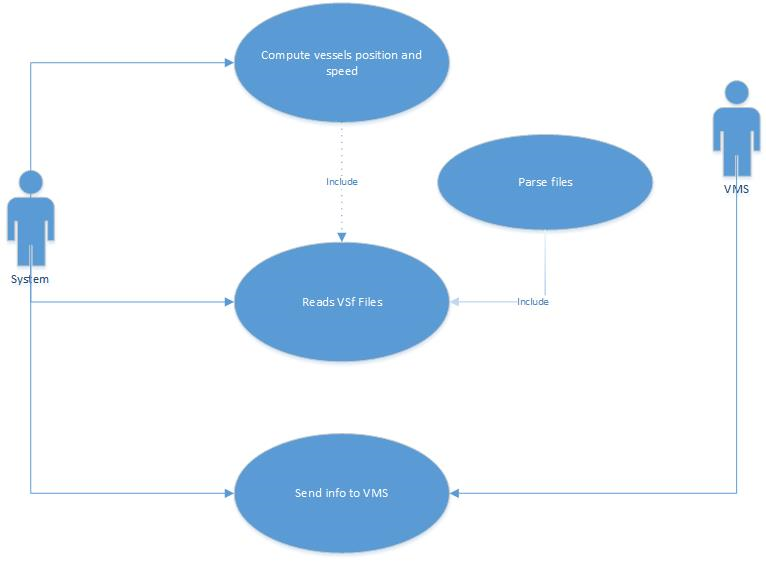
\includegraphics[width=0.8\textwidth]{usecasediagram}
\end{figure}

\noindent
{\bf Name}\\
Radar simulation -Normal Running process

\noindent
{\bf Actors}\\
Vessel monitoring system, Java system

\noindent
{\bf Goals}\\
To send valid vessel information to the VMS

\noindent
{\bf Preconditions }\\
A vsf  file is created and placed in the required locations. 
The file has information on different vessels.

\noindent
{\bf Summary }\\
The radar simulator will read the locations of different types of vessel in a range of 5000 meters,
compute the locations and directions of each vessels, send the different information to the vessel monitoring system, and update every time the vessels change position or location.

\noindent
{\bf steps }\\ 
\begin{enumerate}
\item Open and read the vsf file 
\item Validate the vsf files by checking that there is valid information in the file 
\item Read each line of the file 
\item Disregard any comments that are found in the file
\item Calculate the speed, location, directions, etc.
\item Send the information to the VMS.
\item Repeat steps three to six until the entire file has been read
\item Close the file and quit
\end{enumerate} 

\noindent
{\bf Name}\\
Radar simulation - File not valid 

\noindent
{\bf Actors}\\
Java system 

\noindent
{\bf Goals}\\
To open the vsf file and make sure that it is valid 

\noindent
{\bf Preconditions }\\
A vsf file is created and placed in the required locations.

\noindent
{\bf Summary }\\
The radar simulator will read the locations of different types of vessel in a range of 5000 meters,
compute the locations and directions of each vessels, send the different informations to the vessel monitoring system, update every time the vessels change position or location.

\noindent
{\bf steps }\\
\begin{enumerate}
\item Open the vsf file 
\item Try (and fail) to read the vsf file 
\item Stop the radar simulator and send File Not Found Exception 
\end{enumerate} 
